\chapter{MobCon: A Generative \hyphenation{Middleware} Middleware Framework for J2ME}
\label{ch:mobcon}
\label{ch05}
\mquote{There is abundant evidence to show that high buildings make people crazy.}{C. Alexander et al, Four-Story Limit pattern, A Pattern Language: Towns - Buildings - Construction, Oxford University Press, 1977}

\noindent MobCon\footnote{The name \textit{MobCon} stands for \textit{Mobile Container}.} is a framework\footnote{This chapter shares content with reference \cite{cepa.mezini.hicss38}.} \cite{vasian.mobcon.03} for automating cross-cutting concerns of Java 2 Micro Edition (J2ME) - Mobile Information Device Profile (MIDP) \cite{www.j2me} applications. MobCon uses the technology for attribute-based DSA applied to organize product-lines, introduced in this book. MobCon is implemented as a generative framework that organizes the product-line domain assets as container-managed services specialized for the MIDP development.

\begin{figure}[ht]
%\begin{center}
	  \xymatrix{
	  	*+[F]{\txt{Automating MIDP Applications\\\Sr{sec.mc.Intro}}} \ar[r] \ar[d] & *+[F]{\txt{MIDP Programming with MobCon  \\\Sr{sec.mc.prog}}} \ar[d] \\  *+[F]{\txt{Mobile Container Architecture \\\Sr{sec.mc.arch}}}
	 \ar[r] \ar[d]  	 & *+[F]{\txt{Extending MobCon Framework \\\Sr{sec.mc.extend}}} \\  	
	  *+[F]{\txt{Related Work \\\Sr{sec.mc.rel}}} 	  &   \\	  	
	  }
%\end{center}
%	\caption{Chapter Overview}
%	\label{fig:contents}
\end{figure}

The domain of J2ME MIDP applications is presented in \sr{sec.mc.Intro}. To support a low-cost programming model, a GAAST-like representation is implemented for MIDP. The domain variability is expressed by means of attribute families.

\Sr{sec.mc.arch} represents the details of mobile containers and how they can be used to structure the MIDP product-line domain assets. A comparison of mobile containers with server-side enterprise containers is presented.

MIDP programming with MobCon is explained in \sr{sec.mc.prog}. The declarative programming model introduced by MobCon preserves the model of the domain assets in code and results in shorter development time.

\Sr{sec.mc.extend} gives details about the MobCon internals. Knowledge of the  MobCon internals is needed to extend MobCon. The plug-in meta-data and customization of the transformation workflow are explained. Related container approaches are discussed in \sr{sec.mc.rel}.

\section{Automating Cross-Cutting Concerns of J2ME MIDP Applications}
\label{sec.mc.Intro}

% This section addresses MobCon aspects that are essential to this thesis.  %Other technical aspects of MobCon, e.g., parser implementations for the MIDP code and details of the network protocols, that could be interesting \textit{per se} are explained only when necessary to support the concepts presented in the thesis.

%\subsection{Mobile Software Development with Platform Abstractions: J2EE MIDP}
\label{c2sec:mobile}
\label{c2.j2me}

The development of mobile software has been moving from OEM\footnote{Original Equipment Manufacturer.} specific operating systems and API-s, e.g., Palm OS \cite{palm} and Windows CE / Pocket PC \cite{wce.2003,PocketPC}, to nearly standardized frameworks, e.g., Java 2 Micro Edition (J2ME) \cite{www.j2me} and .NET Compact Framework (.NET CF) \cite{dnet.compact}. The latter aim at offering the same API to application developers independent of the underlying operating system found in the mobile device. J2ME and .NET CF offer an abstraction of the device hardware and software and enable for the mobile software to be portable from one device to another.
% This section gives an overview of mobile software development techniques focusing on mobile device applications that run on virtual machines.
%
The success behind frameworks, such as J2ME \cite{www.j2me} and .NET CF \cite{dnet.compact}, results from the current trend to abstract from concrete hardware execution models by means of \textit{virtual machine} models against which \textit{pseudo-code} is generated. The pseudo-code is then run (compiled, interpreted, compiled just-in-time) in a specific virtual machine specialized for a given mobile device.

The virtual machine execution model introduces an abstraction between the real hardware and particular OEM software on the one side, and the application programs on the other side. The virtual machine abstraction is especially handy for mobile software, where the underlying device hardware and software models change rapidly. It becomes the responsibility of the manufacturer to maintain the specific virtual machine for the manufactured devices. The software applications are mostly isolated from such changes, unless the newly provided features need to be used.

\begin{figure}[ht]
	\begin{center}
		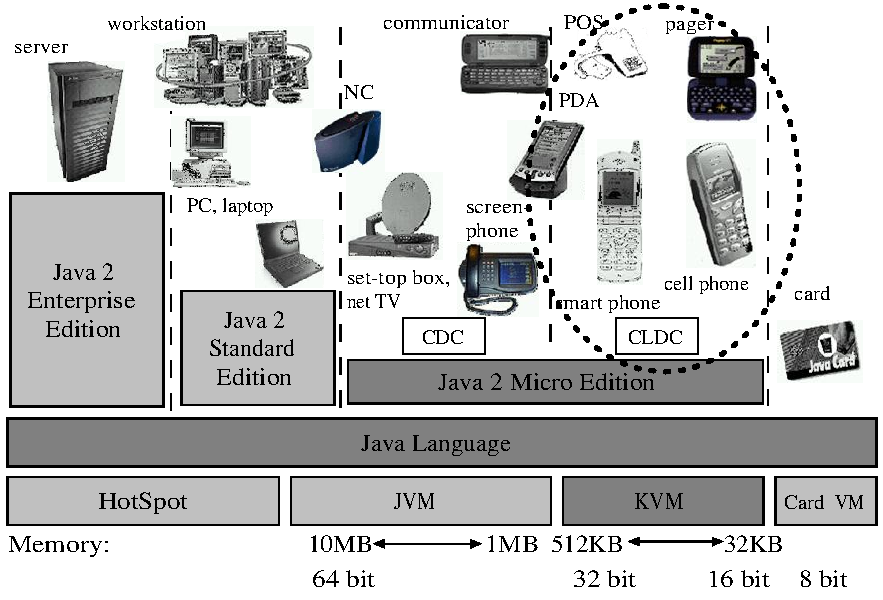
\includegraphics[width=10cm,height=!]{ch02/java}
	\end{center}
	\caption{Java Technologies (Source: http://java.sun.com)}
	\label{fig:java}
\end{figure}

\fig{fig:java} shows the range of the Sun's Java technologies classified according to the targeted devices and hardware technology. Java 2 Micro Edition (J2ME) is the set of Java technologies available for mobile devices. The J2ME technology itself is separated into several families that target different sets of mobile and embedded devices. The most powerful mobile and embedded devices are grouped in \textit{Connected Device Configuration} (CDC) family. The CDC set of devices includes embedded software into TV-Sets, satellite receivers, home video / DVD player devices, powerful PDAs, etc. These devices have enough CPU / RAM resources, power supply sources, and often, constant network connectivity. Standards such as \textit{Open Services Gateway Initiative} (OSGi) \cite{www.osgis}, implemented as \textit{Java Embedded Server} by Sun, target CDC devices that could run some form of the usual Java runtime\footnote{JDK 1.2.}. Scaled down versions of the Java runtime, such as, \textit{Personal Java} profile, could also be used on some of the CDC devices.

Of special interest for this chapter are the devices belonging to \textit{Connected Limited Device Configuration} (CLDC) family. The CLDC family is well supported by Sun and several mobile device hardware vendors \cite{www.j2me.vendors,j2me.2005}. Devices in the CLDC family include, for example, small PDA-s and cellular phones. While PDA-like mobile devices are becoming more and more powerful, the CLDC family will continue to remain in focus as a representative of portable mobile devices. CLDC compatible devices expose many properties usually associated with mobile devices, e.g., limited processing resources compared to other contemporary devices, limited battery life, and sporadic network connections. The CLDC specification is made up of \textit{Mobile Information Device Profile} (MIDP) \cite{www.midp-ota}, whose technology stack is shown in \fig{fig:midp}. MIDP relies on the CLDC virtual machine standard, whose back-end is specialized for the OEM operating system in each device model. The MIDP applications can use the MIDP API-s only and be portable in any CLDC device. Alternatively, MIDP applications can also rely on OEM specific code and be partially portable.

\subsection{The Domain: Automating J2ME MIDP Applications}

The domain addressed in MobCon is that of J2ME MIDP 2.0 \cite{www.midp-ota} applications. J2ME is intended to make programming uniform and simple for mobile devices, following the same goals as Java technology for desktop and enterprise computing \cite{pervasive.java.02}. The MIDP programming model \cite{www.nokia.ep} is based on a very stripped down version of Java. MIDP has a simple language run-time, a simple threading model, and no reflection. The collections and utility libraries are limited to basic types (\texttt{Hashtable}, \texttt{Stack}, \texttt{Vector}). The input / output libraries contain basic stream support. MIDP also contains a set of specialized packages that target CLDC devices. They deal with GUI creation, supporting the idea of a \texttt{Display}, various other input / output gadgets, and game support. It is also possible to play various types of media, e.g., sound or video.

\begin{figure}[ht]
	\begin{center}
		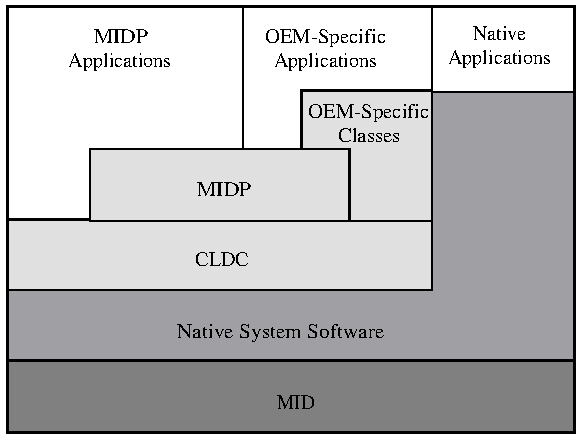
\includegraphics[width=8cm,height=!]{ch02/midp}
	\end{center}
	\caption{MIDP Technology Stack (Source: http://java.sun.com)}
	\label{fig:midp}
\end{figure}

The network communication is supported via a special package for CLDC devices. The basic supported protocols (for MIDP 2.0) include HTTP, HTTPS, UDP, and raw sockets. These protocols are not necessarily supported over TCP/IP. The idea is that any specific device network (packet based) protocol can be used to implement the above protocols and the implementers are free to choose the underlying details. Security is supported via the ability to sign applications and authenticate connections with X.509 certificates. Data persistence is supported via a simple record based model for the local device memory.

A MIDP application is called a \textit{MIDlet}, similarly to a Java applet. A MIDLet should be derived from a specific predefined MIDP class, and should implement a set of required callback methods, e.g., \texttt{startApp()}, that are called by the virtual machine during various phases in the application's life cycle. For an extended and practical discussion about the MIDP programming model the reader is referred to \cite{midp.practical}.

The MIDP technology has proved to be very successful for mobile phones and other small devices, and is supported by many hardware device vendors \cite{lawton.02,www.j2me.vendors,j2me.2005,www.nokia.tp}. There are also good tools and IDE support, and a free reference implementation by Sun. MIDP will be used in this chapter as an underlying technology to demonstrate the concepts represented in this book. 

Despite its simple programming model, MIDP lacks support for modularizing the implementation of \textit{technical concerns}, e.g., data persistence, screen management, session management and security management. These technical concerns \cite{parnas.72} are secondary to what a MIDP application does, but still they must be taken care  explicitly by the developers to get the application running. 
%
When using MIDP, the implementation of secondary concerns cuts across several mobile applications, or even several places within a single application, resulting in duplicated code.
The lack of modularization leads to scattered and tangled code: Not only is the code for technical concerns scattered around several places, it is also tangled with the core functionality. For example, every time the data needs to be saved locally into a mobile device, the \textit{RecordStore} structure that MIDP exposes, needs to be used. The record structure has to be customized manually to match the structure of the data. Similar code is repeated in many places with only very slight differences. The same applies to other concerns, e.g., creating GUI screens and managing the session context.  

The consequence is manifold. First, it makes the development of mobile applications a tedious and error prone task increasing its costs. Furthermore, it is even harder to maintain and further develop such applications, especially in the face of rapidly changing middleware technology for the domain. Given the extreme speed of the domain, it becomes crucial to support off-the-shelf application components that can be reused in a variety of devices. This in turn calls for technology for modularizing technical concerns separately from the application functionality as was explained in \kr{ch02}. 
% it is available for enterprise Java applications, by means of the Enterprise JavaBeans \cite{www.ejb} component model

\subsection{A GAAST-like Representation for MIDP}
\label{mc.gaast}

In \kr{ch03} GAAST-like languages were presented as a prerequisite for introducing low-cost attribute-based DSA to declaratively model the product-line abstractions. The Java dialect supported by MIDP does not support an attribute annotation facility as Java 1.5 does. MIDP also does not support a standard way to access the AST of the parsed MIDP Java code. As the focus in MobCon is in static code transformations, a GAAST-like API for static processing of the MIDP Java code is needed. Adding GAAST-like support to a language is a cheap one-time effort operation. MobCon development was faced with the same problem, to quickly introduce a static GAAST-like representation for the MIDP code. 

The Java dialect of MIDP is similar to Java 1.4. MobCon emulates attributes with JavaDoc \cite{jw-pollac} comments. A special form of JavaDoc comments using an @-sign before the name has been used in several Java 1.4 tools e.g., xDoclet \cite{www.xDoclet} and Attrib4J \cite{java.attrib4j}. When using JavaDoc comments to emulate attributes, no grammar changes need to be introduced in a parser for Java 1.4, apart of the capability to process and preserve the JavaDoc attribute comments. Any tool that parses Java 1.4 could be modified to offer static support for a GAAST-like representation of the source code.

Several third-party generic parsers for Java 1.4 exists, e.g., ANTLR \cite{antlr}, or JavaCC \cite{javacc}. Some specialized Java parsers, e.g., xDoclet \cite{www.xDoclet}, qDox \cite{qdox} have support for processing attributes emulated with JavaDoc comments. Java 1.4 also supports a JavaDoc API that can be used to process JavaDoc comments and could also be used to drive attribute transformations. Unlike full-blown Java code parsers, these tools focus only on parsing  JavaDoc comments and have various limitations in the way they present the Java code. The JavaDoc API, for example, ignores most of the AST information inside methods and cannot be directly used to introduce changes in its model of the Java AST. Other tools, e.g., xDoclet \cite{www.xDoclet} and qDox \cite{qdox}, have similar restrictions. 

\begin{figure}[ht]
	\begin{center}
		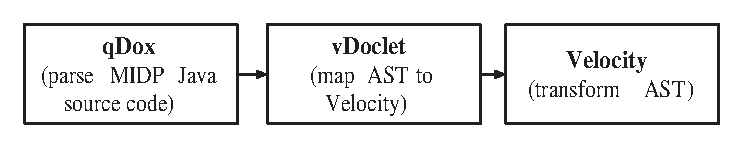
\includegraphics[width=8cm,height=!]{ch05/mobcon-gaast}
	\end{center}
	\caption{MobCon MIDP AST Parsing Tools}
	\label{fig:mc-gaast}
\end{figure}

The qDox \cite{qdox} tool was chosen in MobCon as an underlying tool for creating a GAAST-like representation for MIDP code (\fig{fig:mc-gaast}). There are several, properties that make qDox interesting. As mentioned above, qDox knows how to process JavaDoc style attributes. qDox is also a free open source tool with a very fast parser implementation, which ignores many parts of Java 1.4 syntax. In MobCon, the qDox tool was modified to fully parse MIDP code, that is, to return the method internals as part of the AST and to have support for Java arrays which was not implemented in the original qDox tool. Another very interesting aspect of qDox that motivated its selection in MobCon was the integration of qDox with a tool called vDoclet \cite{vdoclet}. 

The vDoclet tool maps the AST parsed by qDox to a hierarchy of Java objects that can be accessed inside Apache Velocity \cite{velocity} script engine. Apache Velocity is an open source script engine motivated by WebMacro \cite{www.webmacro}, mainly intended for supporting web applications. Using web script engines as meta-programming tools have been explored in many tools, one of the first being Gen\verb@<X>@ \cite{www.genx}. The core of the Velocity is a generic template-like engine that can be used to transform any kind of parameterized source templates. An interesting property of Velocity is that it contains only very basic programming constructs, but allows any Java object to be mapped onto Velocity and accessed directly from the script code. The vDoclet \cite{vdoclet} tool uses this property of Velocity to make the Java AST accessible as native objects in Velocity. The vDoclet tool was also modified in MobCon to reflect the changes that were introduced in qDox. This way, a complete GAAST-like engine was made available in MobCon for transforming the J2ME MIDP applications.

\subsection{Modeling MIDP Attribute Families}


Attribute families were introduced in \sr{attribute.families} as a way to model the variability of the product-line domain assets with attribute-based DSA. MobCon models the generic non-functional MIDP concerns as attribute families. The attributes of the same family are combined with a name space dot-like notation.

\begin{figure}[ht]
	\centering
	\begin{minipage}[b]{5cm}
	\begin{center}	
\begin{footnotesize}
\begin{verbatim}
@src
|- height
|- width
+- form
|  |- label
|  |- firstDisplay
|  ...
|  |- choiceGroup
+- textfield
|  |- label
|  ...
|  |- maxSize
...
\end{verbatim}
\end{footnotesize}
	\end{center}
		\end{minipage}	
	\caption{The MIDP Screen Management Attribute Family}
	\label{mc:scr}

\end{figure}


For example, the attribute family \texttt{@scr}, part of which is shown in \fig{mc:scr}, denotes the screen management concern \see{sec.mobcon.hello}. Inside a family, attributes are distinguished by the family sub-prefix separated by dots. For example, \texttt{@scr.label} denotes the technicalities involved with managing a label gadget within the screen management concern. Many MIDP attributes take arguments that are represented as strings separated by space after the attribute name, e.g., \texttt{@scr.label "First Application"} specifies the text attribute of a label.

End-programmers of the MobCon use the predefined set of MIDP attributes that come with the framework to build mobile applications.  If an attribute is used inside a component (class), MobCon requires that the attribute family name be present to decorate the component itself. The decorated source code is then processed and the required MIDP technical concerns are injected.

\subsection{The MobCon Transformation Engine}
\label{sec.mc.mte}

The \textit{MobCon Transformation Engine} (MTE), illustrated in \fig{fig:mc-mte}, is designed to be a general-purpose transformation framework organized around the modified Java 1.4 parsing tools introduced in \sr{mc.gaast}.

\begin{figure}[ht]
	\begin{center}
		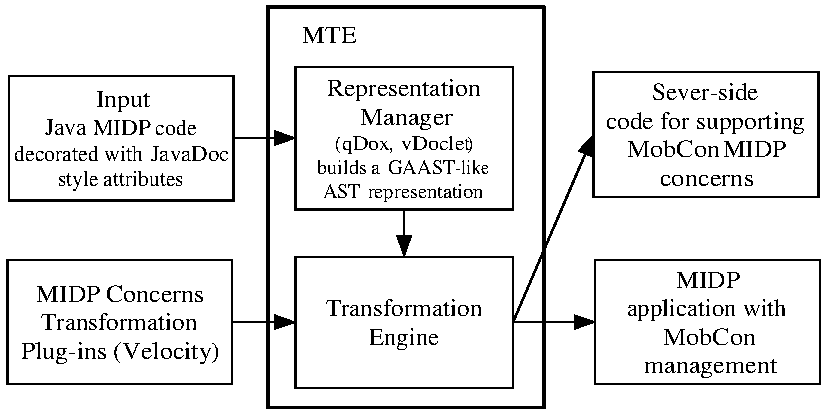
\includegraphics[width=10cm,height=!]{ch05/mte}
	\end{center}
	\caption{MobCon Framework}
	\label{fig:mc-mte}
\end{figure}

The individual MIDP concern transformers are implemented as plug-ins. A plug-in may contain one or more Velocity scripts, Java code, or other resources that describe the plug-in \see{sec.mc.extend}. The MTE contains functionality to properly find plug-in dependencies and manage the transformation workflow \see{sec.mc.wf} by invoking the Java parsing and transformation tools as necessary. Experience with MTE plug-ins was used to develop the Tango attribute-driven transformation framework. Tango and different aspects of building modular attribute-driven transformers processing including those in MTE were discussed in \kr{ch04}.

MobCon relies on the template method pattern \cite{dpatterns} to support well defined extension points \see{sec:ooframeworks}. An abstract class, {\tt AbstractMobApp}, that inherits from MIDP {\tt Midlet} contains the bulk of the generated code. Users do not modify this class directly, since it is modified by the generator each time the attributes in the original source change. Instead, programmers add code to a derived class, {\tt MobApp}, which is called by the abstract class. 
The  template method pattern is useful for generative frameworks \cite{voelter.generation}. It allows programmers to extend the generated code in a modular way without editing it directly.

\subsection{The Mobile Container Architecture}
\label{sec.mc.arch}

\Sr{c2.container.domain} motivated the usage of the software containers as an architectural abstraction to organize the domain assets in software product-lines. \Sr{c2.mobile.container} explained the need to specialize the container concept to address the MIDP domain concerns. One or more mobile client applications run on a mobile device and could connect with server-side services as illustrated in the case (a) of \fig{fig:mob-con-arch}. The server-side part contains functionality that is common to server all clients and functionality specialized for mobile clients, shown by the gray box part in the case (a) of \fig{fig:mob-con-arch}. This specialized client functionality can be factored out from the server part into a separate server-side component known as \textit{adaptive proxy} \cite{fox98adapting}, as in the case (b) of \fig{fig:mob-con-arch}. This separate part is called a \textit{proxy} because it impersonates the server to the mobile clients and vice-versa the mobile clients to the rest of the server (environment) services. It is called an \textit{adaptive proxy} because it does not simply forwards the messages and data from the mobile clients to the server and vice-versa, but also actively modifies the data to adapt them to the specifics of mobile clients. An example of such adaptation is the modification of the resolution of images returned by the server services, to match the resolution required by a mobile device.

\begin{figure}[ht]
	\begin{center}
		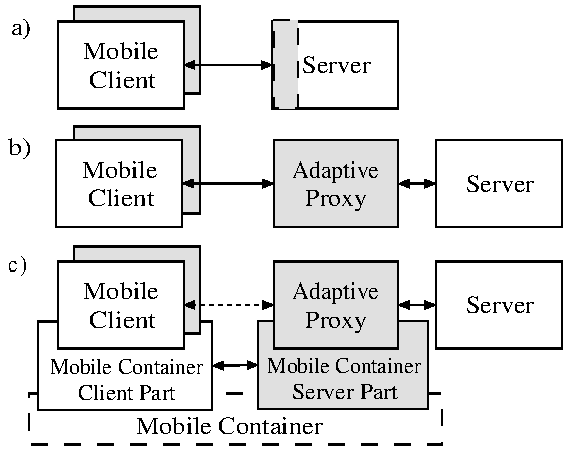
\includegraphics[width=10cm,height=!]{ch05/mc}
	\end{center}
	\caption{The Mobile Container}
	\label{fig:mob-con-arch}
\end{figure}

A mobile container addresses the automation of technical concerns in a mobile application. However, because the functionality of the adaptive proxy part is tightly connected to the functionality of the mobile clients, a mobile container automates both the mobile clients and the adaptive proxy, as in the case (c) of \fig{fig:mob-con-arch}. The mobile client can rely on the container to provide common services specialized for its requirements. In a similar way, in the server-side, the adaptive proxy can make use of the server-part of the mobile container services. The mobile container supported services in both client and server parts are generated and injected based on the requirements of the mobile applications. While a mobile client can still use the server-side services directly, usually it will rely on the mobile container to manage all the communication.

%mob-container
\begin{figure}[ht]
	\begin{center}
		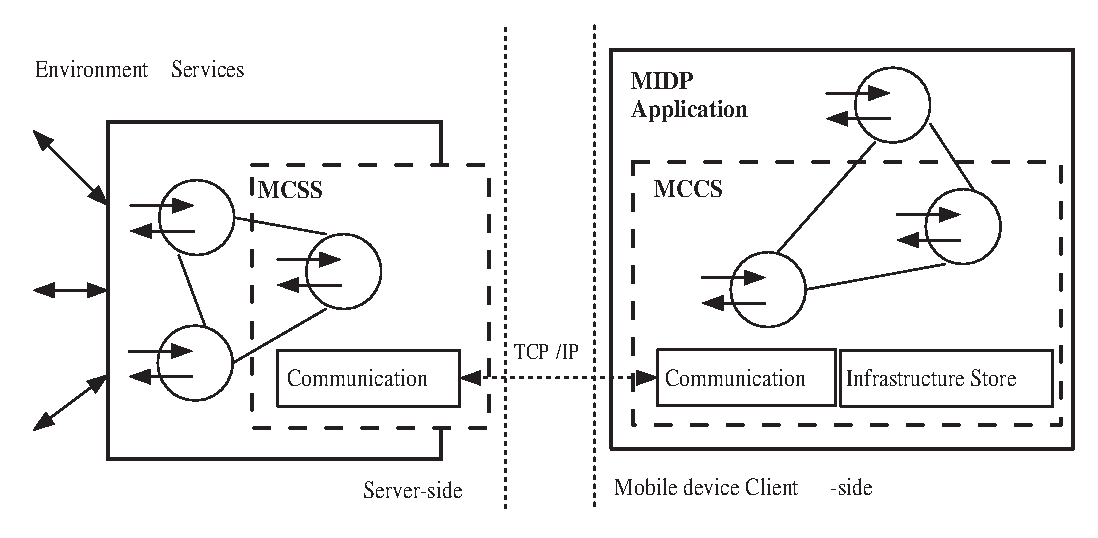
\includegraphics[width=15cm,height=!]{ch05/mobcon}
	\end{center}
	\caption{Mobile Container Components}
	\label{fig:mob-container}
\end{figure}

The conceptual architecture of a \textit{mobile container} is shown in \fig{fig:mob-container}. A mobile container is made of a \textit{client-side} (\textbf{MCCS}\footnote{\textit{Mobile Container Client-Side} part.}) and a \textit{server-side} (\textbf{MCSS}\footnote{\textit{Mobile Container Sever-Side} part.}) part. In the MIDP programming model, the applications cannot share code, including libraries or carry inter-process communication (IPC). This requires to have a MCSS part for every mobile application. It is specialized by generation in MobCon to contain only the functionality needed by the particular application. The MCSS part is instead shared by many mobile clients. It contains generic code in MobCon to identify the clients and fulfill the client-specific requests. The mobile container as a whole manages the communication between the mobile application and the server, and transparently handles the requirements for services by a mobile application. The application specific functionality in both mobile client and the proxy, that is not provided as generic services by the container, is the only code programmed manually by the developers. 

In MobCon, the MIDP transformation plug-ins contain functionality to generate MobCon MCCS code to support the transformed MIDP application, and MCSS code used to support the MobCon concerns in server. The MCSS code must be integrated manually in a server-side application. In MobCon the container is open and extensible. This means that depending on the specific MIDP product-line, developers could add new services to the mobile container needed by server application apart of those already supported by MobCon. This way the mobile container serves as an architectural abstraction \see{c2.container.domain} to organize the MIDP domain concerns in a product-line. This architecture can support at the same time, several families of different domains.

There are more differences between mobile containers and other software (enterprise) containers apart of the explicit separation into two separate physical parts. A mobile container extends from the client device to the server-side. A normal enterprise container works on the server-side and contains some proxy broker code to run on the client. The mobile container does the reverse. The broker-like code is at the server-side. The MCCS part takes care of automation of cross-cutting concerns in a MIDP application running on a mobile device. In an enterprise container, e.g., EJB \cite{ejb21}, the client-side contains only the communication bus and proxy code \cite{server.patterns.02}. The MCCS contains the complete functionality to manage the concerns of MIDP applications. A MIDP application relies on the mobile container to provide the services that map to the required MIDP domain assets. The container manages different aspects of the MIDP application, e.g., the persistence of the mobile application components, and the network communication between the mobile device and the server-side services. Other, more specific domain services, such as image adaptation \see{sec.img.adapt}, are also supported in the same manner as the more generic services by the mobile container \see{c2.container.domain}.

The MCSS part deals with the server-side cross-cutting concerns (CCCs) \cite{parnas.72,kiczalesetal.97}, which are specific for mobile device applications. A mobile device client is different from a desktop client because of the limitations in the processing power, or hardware configuration, e.g., the size of the screen, or the available memory. A mobile device client is neither a thin\footnote{A thin client, here, is an application that contains only the user interface logic and delegates most of the application-functionality processing to the server. A think client does all the data processing itself.} client, because it should be able to work with sporadic network connections, nor it is thick clients since there are usually processing restrictions on the mobile devices. 
The MCSS part addresses mobile device client issues transparently. The interface of the MCSS part to the rest of the server-side services is that of a normal desktop client. The rest of the server-side software in \fig{fig:mob-container} communicates only with the a mobile device client only through the MCSS. The MCSS part contains, thus, more functionality that its symmetrical part in a client of an enterprise container and handles the technical and specific concerns of the adaptive proxy \cite{fox98adapting}.

\section{MIDP Programming with MobCon}
\label{sec.mc.prog}

MobCon is presented to the end-users as a set of attribute-based DSA that support the automation of several technical (and specific) concerns in a product-line for J2ME MIDP applications. The attribute-based DSA modify the semantics of the existing components of a MIDP application. MobCon currently provides MIDP 2.0 support for \textit{data persistence}, \textit{screen management}, \textit{session and context management}, \textit{image adaptation}, \textit{encryption}, and \textit{network communication}. End-users may extend this set of services or modify the existing services \see{sec.mc.extend}. MobCon generates code for the technical MIDP concerns on the client-side (mobile device) and code to be placed on the server-side. The name \textit{MobCon} will be used synonymously with the term \textit{MIDP mobile container} in this section.

A design goal of MobCon is that the attribute decorated code can be used with the manually written parts of the application in a seamless way. The developers can (a) rely on MobCon for the entire application management, or (b) use parts of MobCon for concerns of interests and ignore the others. Developers can use the MobCon generated components or replace them with their own component implementations. MobCon supports an incremental adoption of the MIDP container model inside a specific application. This section presents the MobCon programming model for MIDP applications. First, several MIDP concerns automated by MobCon are presented. Then a complete MIDP application that combines most of the addressed MIDP concerns for a medical X-Ray diagnostics application is explained.

\subsection{Data Persistence}

Any non-trivial MIDP application needs to store data persistently. The non-volatile memory in a MIDP device is organized as a set of record stores managed via the {\tt ja\-vax.mi\-cro\-edi\-tion.rms} package \cite{www.midp}. Each record store is identified by a name unique for a Midlet\footnote{MIDP applications are known as \textit{midlets}, similarly to Java \textit{applets}.}. It contains byte records identified by an integer, the {\tt recordID}. 
%While the {\tt recordID} is incremented when a record is added, the {\tt recordIDs} in a record store may not be consecutive because of record delete operations. 

A MIDP application might need to save data that are too complex to be indexed only by integers. For illustration, consider the \textit{Ga\-me\-Sco\-re} record store example in the documentation of the {\tt ja\-vax.micro\-edi\-tion.rms} package \cite{www.midp}. A \textit{Ga\-me\-Sco\-re} object contains a {\tt player\-Na\-me}, a {\tt score}, and an optional {\tt comment}. Both the {\tt player\-Na\-me} and the {\tt score} fields are used as primary keys. There is no direct way to enable accessing data in a record store for \textit{Ga\-me\-Sco\-re} via arbitrary primary keys. The {\tt ja\-vax.micro\-edi\-tion.rms} package provides support to map arbitrary keys into {\tt recordID}-s by means of enumerating records in a store according to different criteria. The criteria must be coded in a case by case basis for each record store type by implementing two required interfaces: {\tt Re\-cord\-Compa\-ra\-tor} and {\tt Re\-cord\-Fil\-ter}. The {\tt Re\-cord\-Compa\-ra\-tor} defines a partial order over the records in the store, while {\tt Re\-cord\-Fil\-ter} helps to selects certain records.

When using MIDP, a developer must always take care of the store organization details. The store details are intermingled with the application functionality, in the case of the example with the game functionality. This adds significant accidental complexity to the code. This is illustrated by the implementation of a store for the \textit{Ga\-me\-Sco\-re} data which comes with the {\tt ja\-vax.micro\-edi\-tion.rms} package \cite{www.midp} documentation. The code consists in about 216 lines of code of which, as will be shown below (\fig{fig:gamescore}), only about 12\%, belongs to application functionality.  

The increased complexity of the programming model is only one aspect of the problem with a direct approach for implementing the data persistence concern. Other, tightly related issues are maintenance and evolution, which are made more difficult by the lack of the modularity when directly implementing the technical concerns, e.g., data persistence.
Automating the data persistence issues and hiding them from the programmer is highly desirable. Implementing a MIDP store for custom data is a routine operation in a MIDP application and the details are only slightly different from one case to the other.

\begin{figure}[ht]
	\begin{center}
		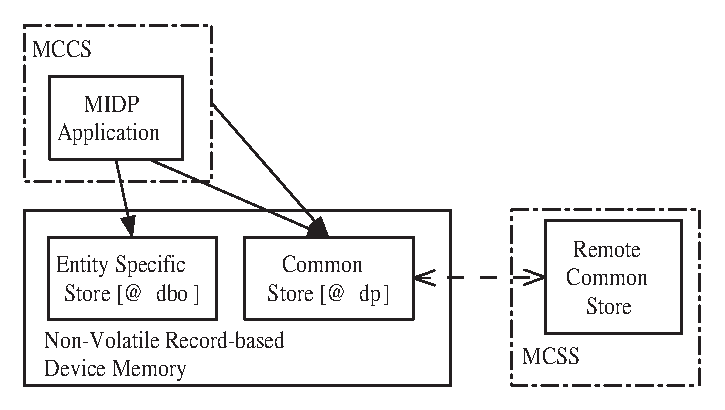
\includegraphics[width=8cm,height=!]{ch05/dp}
	\end{center}
	\caption{MobCon MIDP Data Persistence Architecture}
	\label{fig:mc.dp}
\end{figure}

MobCon addresses data persistence as a technical concern to be factored out by the container and automates store management. The complete data persistence architecture is shown in \fig{fig:mc.dp} and is supported by two attribute families \texttt{@dbo} and \texttt{@dp}. The \texttt{@dbo} family supports specialized stores for components entities. The \texttt{@dp} family supports data persistence in a shared common store. To illustrate the \texttt{@dbo} entity data persistence, \fig{fig:gamescore} shows the complete code for implementing the \textit{GameScore} example in MobCon using the \texttt{@dbo} attribute family, as well as some sample code of how the \texttt{Ga\-me\-Sco\-re} class can be used. 

\newpage
\begin{figure}[ht]
	\begin{center}
		\begin{minipage}[t]{8cm}
		\begin{scriptsize}
\begin{lstlisting}[numbers=left,language=Java,frame=leftline]{}
/**
 * @dbo
 */
public class GameScore {
    /**
     * @dbo.pk
     * @dbo.min 1
     * @dbo.max 256
     * @dbo.sort asc
     */
    private String playerName;
    
    /**
     * @dbo.pk
     * @dbo.min 0
     * @dbo.max 10000
     * @dbo.sort des
     */
    private int score;
    
    /**
     * @dbo.min 0
     * @dbo.max 512
     */
    private String comment;
}
/**
 * @dbo.use GameScore
 */
class GameApp {
  ...
  public void modifyScore(string userName)  {
    GameScore g = GameScore.retrieve(userName);
    ...
    g.setScore(...);
    ...
    GameScore.store(g);
    ...
  }
}
\end{lstlisting}
		\end{scriptsize}
			\end{minipage}
	\end{center}
	\caption{GameScore Example in MobCon}
\label{fig:gamescore}
\end{figure}


The \texttt{@dbo.pk} attributes in \fig{fig:gamescore} are used to denote the primary key fields. The {\tt @dbo.sort} is used to specify how the records should be sorted according to the corresponding field. This information and the field type are used to automatically generate the {\tt Re\-cord\-Com\-pa\-ra\-tor} implementation. The information provided by the {\tt @dbo.min} and {\tt @dbo.max} attributes is used to generate simple validation rules for primitive types\footnote{For integers, the {\tt @dbo.min} and {\tt @dbo.max} attributes specify the allowed lower and upper bounds, whereas for strings they specify the same bounds for the length.}. In addition, an implementation of the {\tt Re\-cord\-Fil\-ter} interface is generated to enable record matching based on the values of primary key fields. Filtering support also includes queries over records by means of the individual primary key fields.

The MobCon implementation of the class \textit{GameScore} in \fig{fig:gamescore} consists of only 27 lines of code, that is, 8 times less than the pure MIDP implementation\footnote{For details about the generated code see \cite{vasian.mobcon.03}.}. Furthermore, the semantics of  the data persistence are declaratively stated in the MobCon implementation, rather than being buried in complicated imperative code for implementing the comparators. The generative MobCon container frees the programmer from having to deal with data persistence details. The programmer uses declarative attribute-based syntax to express the required functionality and can concentrate on the logic that is peculiar to the application. The MobCon framework handles all the details of the data persistence implementation. The attribute-based variability mechanism can also be easily mapped to a graphical wizard, or a visual modeling tool.

\begin{figure}[ht]
	\begin{center}
		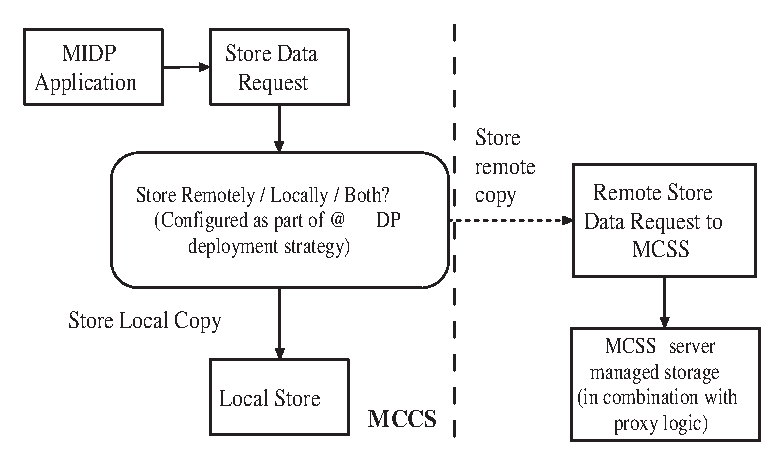
\includegraphics[width=8cm,height=!]{ch05/dpremote}
	\end{center}
	\caption{The \texttt{@dp} Data Store Request Management}
	\label{fig:mc.dp-remote}
\end{figure}

Some mobile applications (or components) might not need a database-like abstraction to persist their data as supported by the \texttt{@dbo} family. A simpler persistence model, in which data is stored as unstructured strings in a hash table structure, i.e., a persistence model more similar to Java serialization, might be good enough. 
%
To support this type of data persistence, MobCon provides the \texttt{@dp} attribute family. Fields annotated with the \texttt{@dp} attribute family are persisted in a shared record store. This common store is also used by MobCon for its internal book-keeping data, e.g., for session and network management. The code needed for performing the data storage is generated by the MobCon framework. 
%
The data of the common store could also be additionally stored remotely on the server, if there is a network connection \see{sec.mc.net}. When the \texttt{@dp} is deployed in a MIDP application, there is a possibility to select between saving all data (a) locally, (b) locally and remotely, or (c) remotely only. These cases correspond to different application scenarios. To explain how MobCon automates remote data storage case consider the logical flowchart of \fig{fig:mc.dp-remote}, which shows how a store data request by a MIDP application is handled by the MCCS part.
 
The deployment case (a) saves all common data locally. In this case the MIDP application stores the data in the mobile device and does not need any remote network connection. The case (b) automatically creates a back-up of the data in server (apart of saving the data locally) when there is a network connection present. When a request for data is made, the local copy is used when no network connection is present. This ensures that the MIDP application can still function reasonably when no network connection is available. The deployment case (c) corresponds to the scenario when the data needs to be saved only remotely, but not locally. This is needed when there is a scarcity of local non-volatile memory in the device, or when the data will be shared and updated by other clients or by the server, and each client needs to operate on the latest copy.

These three scenarios are handled  automatically as part of the \texttt{@dp} deployment. Other scenarios must be currently handled manually. The \texttt{@dp} generated code will take care of establishing the connection to a remote database, if possible, and will perform all the needed actions to persist the common store data for each client on the server-side. Because of the diversity of possibilities for storing data in the server-side (files, different relational databases, XML databases, etc.), MobCon only generates code to manage the store (represented by a \texttt{Tree\-Map}) and serialize data to byte arrays. The developers must add code manually in the proxy to store these data to an appropriate storage organization on the server. In the specific deployment case is known and shared by many applications, then the developers can customize the \texttt{@dp} server-side functionality found in \texttt{Data\-Per\-sis\-ten\-ce\-Trans.ja\-va} file inside the \texttt{@dp} plug-in so that it can be reused by every individual application.

\subsection{Screen Management}
\label{sec.mobcon.hello}

The organization of GUI\footnote{Graphical User Interface.} screens in a mobile application often follows well-defined patterns \cite{www.j2me-ipatterns}. For example, in the \textit{Wizard Dialog} pattern, the user of a mobile application is lead through a series of screens (derived from the class \texttt{Displayable} in MIDP). In this case, it is possible to manage the screen stack automatically, for example, by removing loops, as illustrated in \fig{fig:src.loops}. The screens S2 to S4 in \fig{fig:src.loops} are removed from the stack when S2 is re-shown from screen S4, so pressing the \textit{back} button in screen S2 will show up the screen S1, not S4.

\begin{figure}[ht]
	\begin{center}
$S1 \rightarrow \underline{S2 \rightarrow S3 \rightarrow S4} \rightarrow S2$\\
\textit{remove}
	\end{center}
	\caption{Reducing Loops from the Screen Stack}
	\label{fig:src.loops}
\end{figure}

The MobCon screen management concern takes over the issues related to screen organization and screen stack management. There are attributes in the \texttt{@scr} family to declaratively specify the order of screens, the characteristics of displayed forms, text fields, lists, alerts, and image screens. Common command actions are also taken care by the container implementation of the screen management concern\footnote{More features could be added to this concern in the future, including automatic screen caching and other additional interface gadget combinations.}.

\begin{figure}[ht]
	\begin{center}
	\begin{minipage}{4cm}
		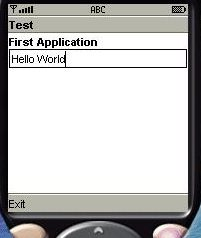
\includegraphics[width=4cm,height=!]{ch05/hellosc1}
	\end{minipage}\hspace{2cm}%
		\begin{minipage}{6.2cm}
		\begin{scriptsize}
\begin{lstlisting}[numbers=left,language=Java,frame=leftline]{}
 /**
  *@scr
  */
 public class MobApp {
   /**
    * @scr.label "Test"
    * @scr.firstDisplay
    * @scr.exitButton
    * @scr.textField textField
    */
   private Form form;
   /**
    * @scr.label "First Application"  
    * @scr.string "Hello World"
    */
   private TextField textField;
 }
\end{lstlisting}
		\end{scriptsize}
			\end{minipage}
	\end{center}
	\caption{MobCon \textit{Hello World} Example Running on a MIDP Emulator}
	\label{fig:hello}
\end{figure}

For an illustration, \fig{fig:hello} shows how a \textit{'Hello World'} MIDP application is programmed using the screen management attributes. The {\tt @scr} attribute attached to the class {\tt MobApp} declares that this class requires the screen management concern.  Only the interface gadget elements are declared as part of the code in the fields {\tt form} and {\tt textField} of the class {\tt MobApp}. Each field element is then decorated with attributes, that declare how it relates to the rest of screen elements. The {\tt @scr.firstDisplay} attribute in line 7 denotes the form that will be displayed first. The form will contain also an 'Exit' button (line 8). The properties of the elements, e.g., their labels, are given as specific attribute arguments.

Most of the repetitive code to be written when a MIDP \textit{midlet} is created, e.g., the required {\tt start} and {\tt destroy} methods, as well as details about implementing the GUI, e.g., the code for creating, customizing and composing the GUI elements, is not explicitly present in MobCon applications. This code is automatically generated by the container. This makes the code involving GUI easier to write and allows the programmer to focus on the core functionality. The interested reader can find the complete MobCon generated code for the simple \textit{HelloWorld} example in \apr{ch.hello.example}. Should the MIDP API-s for managing screen change, the end MobCon based application code does not need to be changed. 

\subsection{Session and Context Management}
\label{sec.mb.session}

Session management is needed in MIDP applications when they communicate with a remote server. The session data support stateful network communication at the application level. For thin clients, it is usually server's responsibility to manage the session data. MIDP applications may want to make use of the possibility to have access to the server session to store their own session data. Related to session management is execution context management, that is, identifying the right mobile device application related to the session data. 

\begin{figure}[ht]
	\begin{center}
		\begin{minipage}[t]{5cm}
		\begin{scriptsize}
\begin{lstlisting}[numbers=left,language=Java,frame=leftline]{}
/**
 ...
 * @ses
 * @ses.rememberLastDisplay
 * @ses.id getMobileID()
 * @log
 * @log.logCommand
 * @log.logMethod
 * @enc
 */
public class MobRay {
 ...
\end{lstlisting}
		\end{scriptsize}
			\end{minipage}
	\end{center}
	\caption{Using Session, Log, and Encrypt MobCon Attribute Families}
\label{fig:mob.ses}
\end{figure}

In MobCon, the context is implemented as a dictionary using a \texttt{Hash\-ta\-ble}. The application can save any data to the context and retrieve them. The session information is saved partially locally, and partially on the server. The session identifier, \texttt{mo\-bi\-le\-ID}, is a unique 128 bit number. This unique ID is assigned to a MIDP application the first time it connects to the server. The \texttt{mo\-bi\-le\-ID} is saved locally by the container for an application in mobile device. The \texttt{mo\-bi\-le\-ID} is reused when the application is reconnected to the server \see{sec.mc.net}. The \texttt{mo\-bi\-le\-ID} serves also as a kind of application \textit{cookie}, which always identifies a particular device instance of a MIDP application. For the session concern, server-side code is generated that handles MIDP sessions and manages the identification based on the \texttt{mo\-bi\-le\-ID} identifiers.

The \texttt{@ses} attribute should be used to decorate the main application class, as shown in \fig{fig:mob.ses}. Predefined support is provided to remember the last displayed form and the unique mobile device session identifier. The session identifier can be changed using the \texttt{@ses.id} attribute. In the example, the parameter of the \texttt{@ses.id} attribute is a code snippet \texttt{get\-Mo\-bi\-le\-ID()} that return the automatically generated \texttt{mo\-bi\-le\-ID}. The \texttt{get\-Mo\-bi\-le\-ID()} is generated by MobCon when the \texttt{@ses} attribute family is used. In a static generative container, such as MobCon, it is possible to use code snippets as attribute arguments. This feature is explored by MobCon to enable the developers to conveniently specify small units of specialization code. 


\subsection{Image Adaptation}
\label{sec.img.adapt}

Mobile devices have limited capabilities so often data, e.g., images, need to be adapted before they are sent to an application that runs on such a device. Images accessed by a MIDP application via a remote server are adapted on the server to match the resolution and colors required by the mobile device. MobCon automatically handles image adaptation using the adaptive proxy pattern \cite{fox98adapting}. The images are stored in their original quality on the server. The MobCon generates code for the MIDP clients as well as for a proxy image adapter to be placed on the server-side. Currently MobCon handles only the MIDP PNG\footnote{Portable Network Graphics.} format images and transforms them on the server-side using JIMI \cite{www.jimi}.

\begin{figure}[ht]
	\begin{center}
		\begin{minipage}[t]{5cm}
		\begin{scriptsize}
\begin{lstlisting}[numbers=left,language=Java,frame=leftline]{}
/**
 * @img.local
 * @img.name "/xrayLocal.png"
 */
 Image ray;
  
/**
 * @img.name getDbe().getImageName()
 * @img.width 100
 * @img.height 100
 * @img.maxcolors 32
 * @img.maxsize 25000
 */
 Image I_ray;
\end{lstlisting}
		\end{scriptsize}
			\end{minipage}
	\end{center}
	\caption{Using Image Attribute Familiy for Static Image Resources}
\label{fig:mob.img}
\end{figure}

The image resource can be either local (stored on the mobile device), or remote and stored in a server. The MobCon \texttt{@img} family can be used to manage the loaded images. The attributes supported by this family allow either decoration of predefined Image objects as shown in \fig{fig:mob.img}, or enable loading images dynamically, by using an automatically generated (overloaded) method:
%Ima\-ge\- re\-trieve\-Ima\-ge(String
%image\-Na\-me,\- int width,\\   int heigth,
%int\- num\-Co\-lors, int\- max\-Size,\- boo\-lean
%di\-ther).

	\begin{center}
		\begin{minipage}[t]{8cm}
		\begin{scriptsize}
\begin{lstlisting}[numbers=left,language=Java,frame=leftline]{}
Image retrieveImage(String imageName, int width, int heigth,
      int numColors, int maxSize, boolean dither){...}
\end{lstlisting}
		\end{scriptsize}
			\end{minipage}
	\end{center}

\begin{figure}[ht]
	\begin{center}
		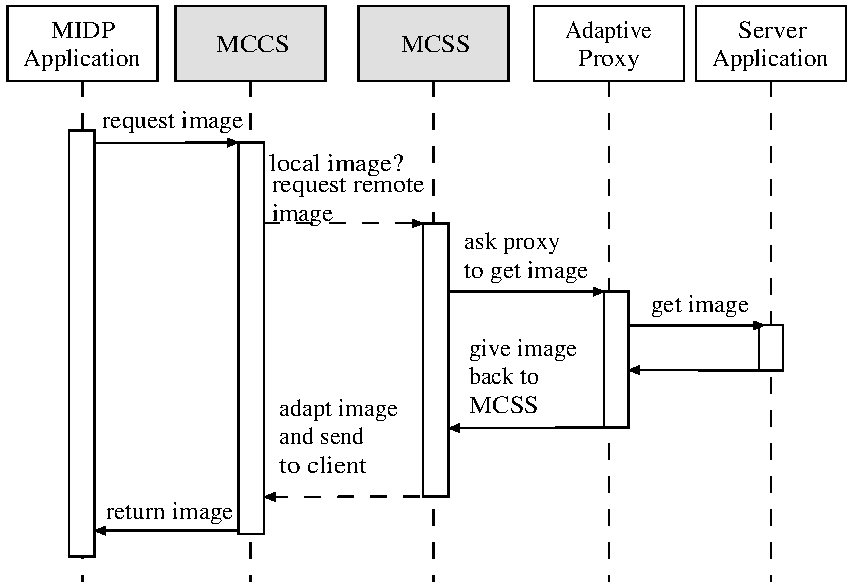
\includegraphics[width=10cm,height=!]{ch05/mc-img}
	\end{center}
	\caption{The Image Request Management}
	\label{fig:mc-img}
\end{figure}

The name of the image will be used to check first for local images, and then for remote images. \fig{fig:mc-img} shows how a request for an image is handled (a UML sequence diagram). First the MCCS part checks to see whether the image is local. If this is the case, MCCS returns the image to the MIDP application. If the image resource is not found locally, a remote request for the image is sent to the MCSS part. MCSS relies on the manual code written in proxy to get the image from the server storage medium of application. The image is then modified in MCSS to match the MCSS request parameters and is returned to the MCCS, which in turn returns the image to the MIDP application. The MobCon implementation of this concern currently does not cache the returned images, as this consumes a lot of memory in the device. MobCon leaves it up to the application to cache the image, e.g., using the managed \texttt{@dp} store as required.

\subsection{Data Encryption}

Currently, the encryption support in MobCon works tightly coupled with data persistence. When data is transfered over the network as part of data persistence, encryption functionality is added to it when required. This enables safe data exchange even when the \texttt{https} protocol is not supported by the MIDP implementation. In the future, encryption could be exposed as a separate concern to be used with network messages. Encryption can be activated application wide using the \texttt{@enc} attribute as shown in \fig{fig:mob.ses}.

When the encryption is activated the data persistence generated methods will be modified to encrypt / decrypt the serialized byte arrays based on an internal key, generated based on the 128 bit unique application \texttt{mo\-bi\-le\-ID} \see{sec.mb.session}. The implementation of encryption concern is based on the third-party {\tt Bouncy\-Castle} \cite{www.bc} lightweight cryptography API for MIDP. A symmetric AES stream cipher in the CFB mode is used to encrypt the network session data.  

\subsection{Network Communication}
\label{sec.mc.net}

Network communication is currently not an explicit separate concern in MobCon. Other concerns, e.g., data persistence and image adaptation, rely on networking support from MobCon, because their implementation is split between the client application and the server-side (\fig{fig:mc.net}). The exact detail of networking support in MobCon are not of direct interest for the scope of this book, so they will be only briefly explained. 

MobCon supports a centralized way to send and receive network messages automatically. This keeps the number of network connections minimum in order to save resources. MobCon can forward any container management message to the appropriate component using a single TCP/IP socket connection. Network messages are by default asynchronous, running on their threads. The network messages are fully identified by:
\begin{enumerate}[a.]

\item A unique MobCon container instance ID (\texttt{mobileID}) in the device corresponding to a MIDP application. This number is used to identify mobile clients and the MCCS requests in the MCSS part, which deals with more than one client at a time \see{sec.mb.session}.

\item A domain asset plug-in ID that is unique for a given domain. That is, each MIDP concern plug-in has a unique ID. This number is used by the MCCS part to identify the concern's plug-in implementation that issues a message. Different concerns define different message subsets, to request different operations from the MCSS. The message subsets of a concern are further identified by the following two numbers.

\item A plug-in instance ID, that is unique for an application instance of the concern, and allows identifying (if needed) the exact component instance that uses the concern.

\item A plug-in dependent operation code, that can be used to carry out commands between the MCCS and the MCSS parts of the container. This code is implementation specific, and is used to specify the meaning of a network message, e.g., whether it is a data store or a data retrieve request.
\end{enumerate}

\begin{figure}[ht]
	\begin{center}
		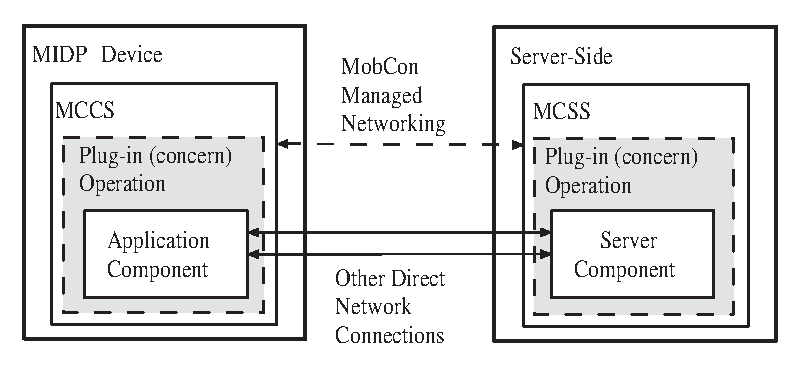
\includegraphics[width=8cm,height=!]{ch05/net}
	\end{center}
	\caption{MobCon Managed MIDP Network Communication}
	\label{fig:mc.net}
\end{figure}

\subsection{Traceability}
\label{sec.mc.trace}

MobCon supports traceability in the same way as discussed in \sr{sec.tango.trace}. Traceability is implemented by a special attribute family \texttt{@log}, that can be used as shown in \fig{fig:mob.ses}. The \texttt{@log} attribute family supports the execution traceability. The execution log lists all MobCon transformers that have changed a given method at run-time as shown in \fig{fig:mobray}. The execution log functionality is implemented as just another MIDP plug-in in MobCon.

\subsection{Case-Study: The \textit{MobRay} Application}
\label{sec.x-ray}

To demonstrate the usefulness of the MobCon framework for the J2ME MIDP applications, a complete use-case application called \textit{MobRay} is implemented. MobRay is based on a ubiquitous X-Ray medical diagnostics scenario \cite{www.xray}. In this scenario, a remotely located hospital uploads X-Ray pictures of patients on its web server and registered doctors use PDA-like devices that run MIDP to review images remotely. Doctors send back to the hospital server their diagnostic comments for the reviewed X-Ray images. The MobRay application was chosen because its implementation demonstrates almost all concerns currently supported by MobCon.

\begin{figure}[ht]
	\begin{center}
		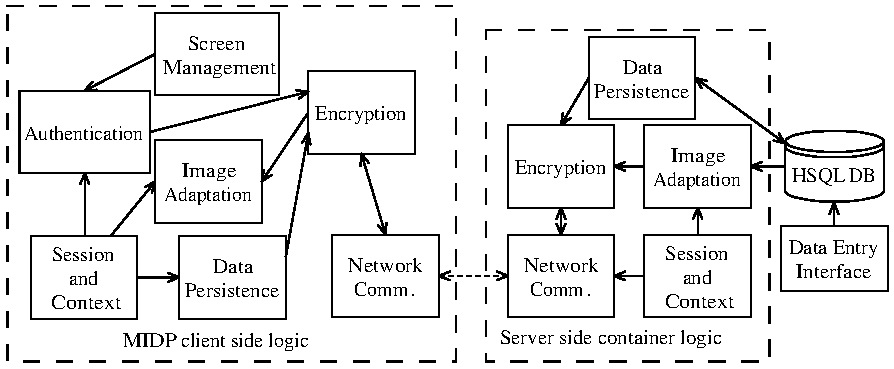
\includegraphics[width=12cm,height=!]{ch05/mobray-struct}
	\end{center}
	\caption{MobRay Application Organization}
	\label{fig:mobray-struct}
\end{figure}

The high-level architecture of the MobRay application and its MIDP concerns are shown in \fig{fig:mobray-struct}. The server-side part of this demo application is implemented using a HSQL database \cite{www.hsql} with a simple command-line interface to allow uploading and editing of patient records. The mobile client-side of the application is developed using MobCon. The client-side contains functionality to connect to the server, to authenticate the doctor and to retrieve the x-ray list to be diagnosed. The x-ray patients lists could then be used to review and send comments on selected x-ray images. The MobCon code for the server-side is placed on a folder called \texttt{server} inside the output folder generated for the MIDP application.
%
The entire client side of the application consists of about 300 lines of MobCon source code (including comments), which then results in more than 1500 lines of code (1:5 ratio) in the generated application. Only the application functionality is explicitly coded. All the named concerns in the boxes of \fig{fig:mobray-struct} are handled by the code generated by the framework. 
%Adding more functionality would be possible but it would not demonstrate anything else about MobCon.

\begin{figure}[ht]
	\begin{center}
	\begin{minipage}{4cm}
		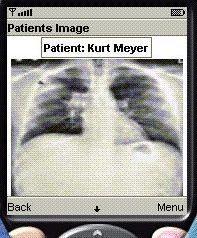
\includegraphics[width=4cm,height=!]{ch05/mobray1}
	\end{minipage}\hspace{0.5cm}%
	\begin{minipage}{8cm}
	\begin{tiny}
	\begin{verbatim}
 mobcon.message.MessageHandler: Getting message from server
 METHOD:  commandAction [@ses, @log]
 COMMAND:  'Select' executed in screen 'Choose a Patient'
 METHOD:  choosePatientCG_Action [@log]
 METHOD:  retrieveEntry [@log]
 mobcon.message.MessageHandler: Getting message from server
 METHOD:  setDbe [@dp, @log]
 METHOD:  callF_patient [@scr, @log]
 METHOD:  callSI_patientName [@scr, @log]
 METHOD:  getDbe [@dp, @log]
 METHOD:  callII_ray [@scr, @log]
 METHOD:  getDbe [@dp, @log]
 METHOD:  retrieveImage [@img, @log]
 mobcon.message.MessageHandler: Getting message from server
 METHOD:  callI_ray [@img, @log]
	\end{verbatim}
	\end{tiny}
	\end{minipage}
	\end{center}
	\caption{MobRay Running on a MIDP Emulator and Part of its Execution Log}
	\label{fig:mobray}
\end{figure}

\fig{fig:mobray} shows a screen shot of the MobRay application along with an extract of its execution log generated by applying the MobCon traceability attribute \texttt{@log} \see{sec.mc.trace}. For example, the method \texttt{callF\_pa\-tient} is modified by the screen concern transformer (as it is tagged by \texttt{@scr}). And of course, all methods effected by logging are modified by the traceability concern transformer \texttt{@log} \see{sec.mc.trace}. 

\section{Extending the MobCon Framework}
\label{sec.mc.extend}

The plug-in architecture of MTE \see{sec.mc.mte} enables several types of extensions: (a) the existing plug-ins can be extended with more services for the MIDP assets they manage, (b) the existing plug-ins can be fully replaced with new MIDP plug-ins, or new plug-ins for new MIDP assets could be added, (c) an entirely new set of plug-ins to support a container for a new domain based on Java 1.4 can be introduced. In all the cases, the domain assets are modeled as attribute-based DSA, which removes the need to modify the grammar of the original language. In order to apply successfully the attribute-based DSA and to be able to extend MobCon the transformation details need to be understood. The transformation workflow should be chosen based on the semantics of the domain assets. \Kr{ch04} discussed all these concepts in a generic level based on the Tango framework. This section only explains details specific to the current implementation of the MobCon framework, noting differences between MTE and Tango as necessary. More information can be found in the MobCon documentation \cite{vasian.mobcon.03}.

\subsection{Workflow and Plug-in Metadata}
\label{sec.mc.wf}

A MobCon plug-in is packed as a Java JAR file whose structure is shown in \fig{mc:scr-dirs}. The plug-in JAR file contains, among  other files, a manifest file with custom entries that describes the plug-in meta-data. An example of a manifest file for the session management (\texttt{@ses}) plug-in is shown in \fig{fig:mc.manifest}.

\begin{figure}[ht]
	\centering
	\begin{minipage}[b]{5cm}
	\begin{center}	
\begin{footnotesize}
\begin{verbatim}
<session>
|- MANIFEST.MF
+- <jar>
   |- session.tag
   |- session.vm
   |- ... 
\end{verbatim}
\end{footnotesize}
	\end{center}
		\end{minipage}	
	\caption{The \texttt{@session} Transformer Organization}
	\label{mc:scr-dirs}

\end{figure}

\begin{figure}[ht]
	\begin{center}
	\begin{minipage}[t]{6cm}
		\begin{scriptsize}
		\begin{lstlisting}[numbers=left,language=Java,frame=leftline]{}
Manifest-Version: 1.0

name: Transformer
Transformer-Name: Session
TID: 04
IID: 01
File-Name: session.vm
Tag-File: session.tag
Server-File: SessionTrans

name: Dependencies
Use-Before: 02.01
Use-After: 		
		\end{lstlisting}
		\end{scriptsize}
		\end{minipage}
	\end{center}
	\caption{The \textit{MANIFEST.MF} file for the \textit{Session} Plug-in}
	\label{fig:mc.manifest}
\end{figure}

The manifest file contains several sections identified by the different \texttt{name:} labels in lines 3 and 11 of \fig{fig:mc.manifest}. There is a user friendly transformer name in line 4. The transformation ID (TID) in line 5 identifies the domain concern that the plug-in transformer supports, in this case the session management. The next number, the plug-in instance ID (IID) is the number given to the actual implementation of this plug-in \see{sec.mc.net}. MobCon enables using more than one possible implementation for a given TID in an application, or more often, in different applications. The main Velocity script file of the plug-in transformer is specified in line 8. When the transformer generates also serve-side code (Java SDK 1.4 is used for server-side code), then the line 9 specifies the names for the generated server-side files. The dependencies section, in lines 10 to 13, defines the default plug-in dependencies explained in \sr{sec.workflow}. While user-friendly names can be used, MobCob requires unique identifiers in the form TID.IID to be used in the dependency lists.

\begin{figure}[ht]
	\begin{center}
	\begin{minipage}[t]{6cm}
		\begin{scriptsize}
		\begin{lstlisting}[numbers=left,language=XML,frame=leftline]{}
<flow>
    <group>
        <transformer>
            <name>Screen</name>
            <tid>02</tid>
            <iid>01</iid>    
            <merger>
                <class>MixTemplateExample</class>            
            </merger>
        </transformer>
        <transformer>
            <name>Mix Example</name>
            <tid>07</tid>
            <iid>01</iid>
        </transformer>      
    </group>
...
		\end{lstlisting}
		\end{scriptsize}
		\end{minipage}
	\end{center}
	\caption{MobCon Dependency File}
	\label{fig:mc.dep}
\end{figure}

As explained in \sr{sec.workflow}, the global transformation workflow is calculated automatically in MobCon based on the local plug-in meta-information found in the \textit{MA\-NI\-FEST.MF} file. This frees the developers from having to create the total dependency graph manually. In the MIDP case, the existing plug-in dependencies are specified in their corresponding manifest files. If a new plug-in is added or an existing plug-in is modified or replaced, the plug-in manifest file must be edited to reflect the new order. MobCon supports also an application specific order, where each application can override the workflow order by modifying the \texttt{lib$\backslash$plugins$\backslash$de\-pend.xml} dependency file generated by MobCon inside the application directory. For example, the dependency file of \fig{fig:mc.dep} has been modified to support a custom combination of the output of the \textit{Screen} transformer (line 4) and a custom \textit{Mix Example} transformer (line 12), by using a custom mixer \texttt{Mix\-Tem\-pla\-te\-Exa\-mple} transformer (line 8). A mixer transformer must implement the \texttt{Mix\-Tem\-pla\-te} interface of \fig{fig:mix}. \Kr{ch04} discussed how this concept is generalized in Tango to mix an arbitrary number of classes at the same time.

\begin{figure}[ht]
\begin{center}
\begin{minipage}{12cm}
\begin{scriptsize}
\begin{lstlisting}[numbers=left,language=Java,frame=leftline]{}
public interface MixTemplate {
  public ClassTemplate 
     mixClasses(ClassTemplate ct1, ClassTemplate ct2);
  public MethodTemplate 
     mixMethods(MethodTemplate mt1, MethodTemplate mt2);
}	
\end{lstlisting}
\end{scriptsize}
\end{minipage}
\end{center}
\caption{MobCon MixTemplate Interface}
\label{fig:mix}
\end{figure}

Apart of the dependency meta-data a plug-in file contains also a tag dictionary file (\texttt{.tag}). The tag dictionary is a Java property file that maps the attribute names used in source code to those used by the plug-in internally. This allows developers to customize the attribute names used in code. For example, instead of \texttt{@dp} they could use \texttt{@da\-ta\-Per\-si\-sten\-ce} in code. The plug-in implementation treats the attribute names as string resources: \texttt{\$class.\-get\-Tag(\$tag\-Dic.\-get\-Tag("dp"))}. The trace log will use whatever name the user choses for the attributes.

\subsection{Transformation Details}

MobCon plug-ins use the Apache Velocity \cite{velocity} script engine to manipulate the code. The default mode for the Velocity engine is to output text using the Java \texttt{System.out} object. The MTE modifies the Velocity initialization not to output code directly. Instead, MobCon makes accessible for modification to the Velocity scripts, a set of GAAST-like class template API (CT-API) as explained in \sr{sec.ast.tango}. Working with the CT-API facilitates many aspects of the transformer implementation, that would need to be expressed as text Velocity templates otherwise. The vertical attribute-driven transformer modularization explained in \sr{sec.tango.layers} is not supported in MobCon. For an example of how a transformation can be implemented in MobCon, consider the attribute-decorated code of \fig{fig:mc.code}.

\begin{figure}[ht]
	\begin{center}
	\begin{minipage}[t]{6cm}
		\begin{scriptsize}
		\begin{lstlisting}[numbers=left,language=Java,frame=leftline]{}
 /**
  *@scr
  *@dp
  */
  public class Test{
  . . .
 /**
  * @dp.access
  * @scr.store
  */
  private String id;
		\end{lstlisting}
		\end{scriptsize}
		\end{minipage}
	\end{center}
	\caption{Example MIDP Input Code}
	\label{fig:mc.code}
\end{figure}

\fig{fig:mc.code.vs} shows a part of a transformer implemented in Velocity that processes the \texttt{dp.access} tag in \fig{fig:mc.code}, referred by the name \textit{"accessible"} in the tag dictionary (line 3). A Velocity macro \texttt{dp\_\-meth\_\-get} (lines 9, 16) is used to generate the code in line 5. Inside the macro, a class template object that represents a method is created and mapped as a Velocity object (called a \textit{bean}) by using the vDoclet tool (line 10 in \fig{fig:mc.code.vs}). The method template object is then modified by the macro to customize it to model an accessor method. 

\begin{figure}[ht]
	\begin{center}
	\begin{minipage}[t]{10cm}
		\begin{scriptsize}
		\begin{lstlisting}[numbers=left,language=Java,frame=leftline,showstringspaces=false]{}
#foreach ($field in $class.fields)
  #set($tag = false)
  #set($tag = $field.getTag($tagDic.getTag("accessible")))
  #if ($tag)
   #dp_meth_get($field.type $field.name)
  #end
. . .

#macro(dp_meth_get $type $name)
 #set($MT = $vdoclet.makeBean("mobcon.ct.MethodTemplate"))
 $MT.setAccess("public")
 $MT.setType("$type")
 $MT.setName("get$StringUtils.capitalizeFirstLetter($name)")
 $MT.addEnd("return $name;")
 $CT.addMethod($MT, $tagDic.getPrefix())
#end
		\end{lstlisting}
		\end{scriptsize}
		\end{minipage}
	\end{center}
	\caption{Example Velocity Script for Processing \fig{fig:mc.code}}
	\label{fig:mc.code.vs}
\end{figure}

\noindent The generated code for the accessor method looks as in \fig{fig:mc.code.vs.out}, where a method named \texttt{get\-Id()} is generated. \Kr{ch04} discussed how attribute-based transformers can be further modularized to scale the transformation.

\begin{figure}[ht]
	\begin{center}
	\begin{minipage}[t]{5cm}
		\begin{scriptsize}
\begin{lstlisting}[numbers=left,language=Java,frame=leftline,showstringspaces=false]{}
. . .
  public String getId(){
    return id;
  }
. . .
		\end{lstlisting}
		\end{scriptsize}
		\end{minipage}
	\end{center}
	\caption{Example Output Code for Example of \fig{fig:mc.code}}
	\label{fig:mc.code.vs.out}
\end{figure}

\section{Related Work}
\label{sec.mc.rel}

\Sr{sec.c2.ejb} discussed the J2EE containers and explained that EJB \cite{ejb30} is moving toward a simpler programing model based on attributes. The motivation to use attributes in EJB is not to support a low-cost DSA mechanism. Rather, a predefined specific set of attribute-based DSA is used as a clear and uniform way to support the EJB programming model for enterprise containers. The current version of the latest EJB specification is not fully-completed and leaves the discussion open for feedback in some places, on what is the best way to support a concern, or how to express it better with attributes. MobCon is an open attribute-driven framework for supporting arbitrary attribute-based containers. MobCon is specialized with a set of plug-ins for MIDP applications. The set of attributes that can be used to support a product-line is left open and MobCon enables experimentation. The transformation workflow is customizable and can be modified on a per application basis. The source code parsing engine of MobCon supports a Java 1.4 compatible syntax, similar to the one found in MIDP and has not support for Java 1.5 style annotations\footnote{The AST representation manager could be replaced, if needed, in MonCon to enable Java 1.5 support. The new AST needs to be mapped similarly to vDoclet \cite{vdoclet} tool. These issues are outside the focus of this book. The current MIDP Java dialect syntax is very similar to the Java 1.4.}.

The SmallComponents \cite{www.smallcomps} approach is based on generative techniques and visual modeling to introduce a logical container abstraction. SmallComponents address embedded systems, where the size of the middleware must be optimized with respect to specific application needs. To achieve this goal, an adaptable container abstraction is used as a replacement for the middleware itself. SmallComponents is based on graphical domain-specific languages (UML), rather than on attributes. The SmallComponents approach addresses embedded and real-time systems, where generative approaches are superior to other code abstraction techniques. In MobCon, the container abstraction is not seen as a replacement for the mobile middleware. It rather augments the MIDP middleware with convenient software abstractions to make the MIDP applications easier to develop and maintain. Attributes support a modeling-like view, directly at the source level \see{sec:var.dsa}.

There are many source-to-source transformation and meta-programming approaches and frameworks available \cite{generative.00}. The MobCon transformer framework is specialized for building attribute-driven source code transformers, which may need to be maintained often, to reflect changes in the underlying middleware. Unlike other Velocity-based \cite{velocity} transformers \cite{www.velocity.powered,www.AndroMDA}, MobCon transformers do not use Velocity directly to output code, but rather work on the specialized GAAST-like API \seec{ch03}. This makes it easier to support code generation in the case of cascaded transformers. The effects of attribute-driven transformation and their relation with other transformation approaches were discussed in \kr{ch04}.

Adaptive proxies \cite{fox96adapting,fox98adapting} enable transparent access of server-side services from a mobile client. They stand between the server-side application and a mobile client application, and dynamically adapt the server data requested by the mobile client in order to fit to the capabilities of the mobile client device. The adaptive proxy can reside in the same machine as other server-side services, or in a separate machine. 
MobCon automates the technical concerns of the adaptive proxy related to the mobile application. The server-side part of a mobile container transforms the data to prepare them for the mobile device. MobCon generates the server-side part based on the requirements for the container concerns support in the client-side part. These services are used then by the adaptive proxy functionality.

Aspect-oriented programming (AOP) \cite{kiczalesetal.97} techniques discussed in \sr{ch2:aop} can also be used to support attribute-driven transformations \cite{aop.attrib.05}, and to achieve independence from specific middleware \cite{aop.middleware.03}. AOP tools, e.g., AspectJ \cite{Laddad.aop, www.aspectjt} can be used in two ways to support transformations enabled by MobCon. (a) AOP-style factorizations based on the description of the component joinpoints as pointcuts (implicit hooks \cite{java.compost}) can be used. This is the only available technique in AspectJ before the support for Java 1.5 annotations. This indirect style of programming requires redefining the pointcuts for every component that needs container support, in every specific application, in order to match the advice code. (b) AOP tools can be used to work upon attributes (explicit hooks \cite{java.compost}) as a generic meta-programming engine \see{sec.aop.dsa}. AOP techniques require also some form of run-time support (added statically by AspectJ) to support the pointcut context management. This infrastructure would be appended to the infrastructure code required by the mobile container. The duplicated infrastructure would result in more overhead than with other meta-programing techniques that maintain the node selection context explicitly during the transformation.

AOP techniques could be also supported completely at run-time with additional run-time support. In \cite{aop.da.02} dynamic AOP techniques are used to implement context adaptable sockets. In \cite{spont.container} \textit{spontaneous containers}, based on dynamic AOP, are used along with Jini \cite{www.sunjini} to adapt mobile applications to several environment services. These approaches support for dynamic services. Dynamic AOP techniques are too heavy for MIDP applications and require a more powerful class of devices. For example, MIDP currently does not support programmable code downloading and has no reflection capabilities\footnote{Therefore, Jini \cite{www.sunjini} cannot be used.}, which makes such techniques not applicable. For this reason, the MobCon approach presented here deals only with static transformations of the J2ME MIDP 2.0 applications.

\cendsection{Chapter Summary}

MobCon is a framework for automating technical concerns of MIDP 2.0 applications built upon the concepts introduced in this book. J2ME MIDP applications exhibit repeated cross-cutting functionality that can be factored out from one or more applications. This common functionality can be parameterized and made part of  product-line to support MIDP applications. 

It is preferable to express the MIDP domain assets declaratively in source code. The programmers concentrate on the specific application functionality and express the cross-cutting concerns declaratively. Attribute-based DSA provide a low-cost mechanism for supporting a customizable declarative programming model. A GAAST-like representation of the MIDP Java source is realized based on several open-source tools. These tools allow manipulation of JavaDoc-like decorated source code.

MobCon's programming model is based on the decoration of program entities with attributes. The variability of the technical MIDP concerns is modeled as attribute families. Each family is specialized for a given concern, and contains nested levels of sub-families to express different aspects of the variability. Finally, attribute arguments are used to parameterize the attribute families.
%
The MobCon Transformation Engine (MTE) is organized around the attribute families and employs the different transformation units as plug-ins. MTE contains functionality to drive the transformation workflow based on the plug-in dependencies. The template method pattern is used to separate the generated and manually entered code.

Mobile containers are a special kind of client container specialized to automate the concerns of product-lines for mobile applications. A mobile container automates not only the software running in the client mobile device, but also the related part of software into the server-side. Mobile containers offer an architectural abstraction to organize the domain assets of MIDP product-lines.

Several attribute sets are predefined and automate concerns related to J2ME MIDP, e.g., the persistence of data in the mobile device or across the network. The implemented concerns were selected to be representative of common MIDP tasks, which show up repetitively in many MIDP applications. A case study based on an application for medical X-Ray diagnostics was shown. The addressed MIDP concerns are injected automatically into the X-Ray application, resulting in less code, focusing only to the specific functionality.

The concerns currently addressed by MobCon are by no means a complete set covering every possible MIDP application. The MobCon attribute-driven transformation engine is extensible and allows new plug-ins to be defined and integrated into a container. Plug-ins represent one or more transformers specialized for a specific concern. New plug-ins could add more MIDP services, or provide support for a totally different domain. The generative framework itself is written in Java and is independent of the plug-ins functionality. The transformation control flow is determined based on the declared plug-in workflow preferences, and can be overwritten manually for specific cases.

 
%Some MIDP applications such as games require hand-made optimizations customized to a particular solution. Even general applications can use some of these optimization usually based on compression techniques, such as those mentioned in \cite{optim.midp.02}. In \cite{cepa.netz} we have investigated run-time decompression of .NET assemblies. In the future, such optimizations cloud be made part of the MobCon framework concerns.
